%\documentclass[preprint, review, 3p, authoryear]{elsarticle}
\documentclass[10pt, a4paper]{article}

%\usepackage{setspace}
\usepackage[utf8]{inputenc}
\usepackage{amsmath, amssymb, amsthm, bbm}
\usepackage{xcolor}
\usepackage{graphicx}
\usepackage[authoryear]{natbib}
\usepackage{apalike}
\usepackage{relsize}
\usepackage{array}
\usepackage{multirow}
\usepackage{showlabels}
\usepackage{setspace}

\DeclareMathOperator*{\argmax}{arg\,max}

\newtheorem{prob}{Problem}
\newtheorem{prop}{Proposition}
\newtheorem{definition}{Definition}

%%%%% bold symbol in math enviornment
\newcommand{\m}[1]{\boldsymbol{#1}}

\title{Merging the components of a finite mixture using  posterior probabilities}
\author{M. Comas-Cufí \and J.A. Martín-Fernández \and G. Mateu-Figueras}

%\doublespacing
\begin{document}

\maketitle

\section{Introduction}

%Cl
The most standard parametric approach in cluster analysis assumes data can be modelled by a finite mixture distribution. The approach has two steps; first, a finite mixture distribution with probability density function
\[
f(\;\cdot\; ; \pi_1, \dots, \pi_k, \m\theta_1 \dots \m\theta_k) = \pi_1   (\;\cdot\; ; \m\theta_1) + \dots + \pi_k f(\;\cdot\; ; \m\theta_k),
\]%
%with $\sum_{j=1}^k = \pi_j =1$
is fitted to a sample $\m X$, obtaining estimates $\hat{\pi}_1, \dots, \hat{\pi}_k$ and $\hat{\m\theta}_1 \dots \hat{\m\theta}_k$. After the fitting process, each observation $\m x$ is assigned to the finite mixture component $j$, $1\leq j \leq k$, with $\hat{\pi}_j f(\m x ; \hat{\m\theta}_j)$ maximum. 

In the previous approach, it is common to have mixture components not separated enough from other mixture components, and therefore, it is difficult to consider them as two different cluster. To deal with this situation, different authors propose to consider two or more components to form a unique cluster, and therefore, to combine or to merge different components into one single component ({\color{red} Cites rellevants per el problema d'ajuntar components. Preparar llista actualitzada i afegir les cites segons la revista on es decideixi enviar}).

In \cite{hennig2010methods} the author reviews different approaches and separates the existing approaches in two different groups: those methods based in modality and those methods based on misclassification probabilities. 

All methods described in this paper are based on posterior probabilities, $\hat{\tau}_{ij}$, that an observation $\m x_i$, $1\leq i \leq n$, is generated by component $j$, $1\leq j\leq k$ \citep{longford2014,melnykov2013distribution,hennig2010methods,baudry2010combining}. All this methods can be included inside the category of methods based on misclassification probabilities. Although this approaches have been presented for Gaussian mixtures, the fact that they are based only on the posterior probabilities allow us to apply each method using any other probability distribution mixtures.

In this paper we review and introduce different approaches to combine the finite mixture components using posterior probabilities. Moreover, we introduce a general formulation for such methods which allow us to introduce a new family of methods to solve the same problem.

The paper is organised as follows: In Section~\ref{definitions} we introduce two concepts; \emph{the partition of a finite mixture distribution} and \emph{the hierarchical combination of components}. The definitions are going to be useful to standardise notation between different methods. We show a simple example to get used to the new notation. In Section~\ref{old_methods}, the approaches to obtain a hierarchical combination of components appeared in \cite{hennig2010methods} and \cite{baudry2010combining} are presented using the new notation. 

%Moreover, a new method based on log-ratios is introduced. In Section~\ref{confusion} the problems a reformulated in a common approach, they are compared to the approach presented in \citep{longford2014} 


%In general, \cite{hennig2010methods} summarises the algorithm of hierarchically merging Gaussian components as follows:
%\begin{enumerate}
%\item Start with all components of the initially estimated Gaussian mixture as current clusters
%\item Find a pair of components to merge and forming a single cluster
%%\item Calculate the posterior probability of pertinence to a cluster 
%\item Apply a stopping criterion to decide whether to merge them to form a new current cluster, or to use the current clustering as the final one.
%\item If merged, go to 2.
%\end{enumerate}

%As commented, in this paper we only focus on methods based on the posterior probabilities. Our aim is to find strategies to hierachically merge components into clusters. Let us remark that we will not focus on stopping criteria, and therefore we will hierarchically merge all components until a single cluster with all components is obtained.




% \section{The subjectiveness of clustering decisions}
% 
% It is well known that there is a strong subjective component in the decision of what a ``true cluster'' is \citep{hennig2010methods}.
%
% \begin{prob}
% Given a compositional sample $T = \{ \boldsymbol{\tau_1}, \dots, \boldsymbol{\tau_n} \}$, with $\boldsymbol{\tau_i} = (\tau_{i1}, \dots, \tau_{iK})$ denoting the pertinence to classes $C_1, \dots, C_K$, build a hierarchy over the set of classes.
% \end{prob}

\section{Definitions}
\label{definitions}

Let $\mathbb{X}$ be a sample space. A \emph{finite mixture of distributions} is a probability distribution with probability density function (pdf) defined as the linear combination of pdf from other probability distributions defined in $\mathbb{X}$. In general, the pdf $f$ of a finite mixture of distributions is
\begin{equation}\label{mixt}
f(\;\cdot\; ; \pi_1, \dots, \pi_k, \m\theta_1 \dots \m\theta_k) = \pi_1 f_1(\;\cdot\; ; \m\theta_1) + \dots + \pi_k f_k(\;\cdot\; ; \m\theta_k),
\end{equation}
where $\m\theta_1, \dots,  \m\theta_k$ are the parameters of the pdf $f_1, \dots, f_k$ respectively and, because $\int_{\mathbb{X}}f = 1$ the restriction $\sum_{\ell = 1}^k \pi_\ell = 1$ holds. The pdf's $f_1, \dots, f_k$ are called the \emph{components} of the finite mixture $f$, or simply the \emph{mixture components}.

Let $f$ be a finite mixture of distributions with  parameters  $\pi_1, \dots, \pi_k, \m\theta_1 \dots \m\theta_k$ as defined in Equation~\ref{mixt}, and let $I$  be a subset of $\{1, \dots, k\}$. We denote by $f_I$ the finite mixture of distributions with pdf defined by
\[
f_I = \sum_{j \in I} \frac{\pi_i}{\pi_I} f_j(\;\cdot\; ; \m\theta_j)
\]
where $\pi_I = \sum_{\ell \in I} \pi_\ell$. To simplify, we do not specify the parameters of $f_I$, which are parameters borrowed from $f$. Note that using this notation, we have that $f_{\{1, \dots, k\}} = f$ and $f_{\{j\}} = f_j$.

A \emph{partition} $\mathcal{I}$ of $\{1, \dots, k\}$ is a set of subsets of $\{1, \dots, k\}$, called $parts$, such that $\bigcup_{I \in \mathcal{I}} I = \{1, \dots, k\}$ and  if two parts $I, J \in \mathcal{I}$ are different, $I \cap J = \emptyset$ holds. To simplify, through this paper we assume an order within the elements of a partition. Doing so, we can index the partition and write $\mathcal{I} = \{ I_1, \dots, I_s\}$. It is important to note that given any partition $\mathcal{I} = \{ I_1, \dots, I_s\}$ of $\{1, \dots, k\}$, the mixture $f$ (Eq.~\ref{mixt}) can be rewritten as
\begin{equation}
f = \pi_{I_1} f_{I_1} + \dots + \pi_{I_s} f_{I_s}.
\label{mixt_part}
\end{equation}


A \emph{hierarchical combination of components} is a sequence of partitions $\mathcal{I}_1, \dots, \mathcal{I}_k$ of $\{1,...,k\}$, where $\mathcal{I}_1$ is the one-part partition $\mathcal{I}_1 = \{ \{1, \dots, k\} \}$, and for each $k'$, $1 <  k' \leq k$,
\begin{itemize}
\item $\mathcal{I}_{k'}$ has $k'$ elements  and
\item if a part $I \in \mathcal{I}_{k'-1}$ then either there is a part $J \in \mathcal{I}_{k'}$ with $J = I$ or there are two parts $J_1, J_2 \in \mathcal{I}_i$ with $I = J_1 \cup J_2$.
\end{itemize}


\subsection*{Model-based clustering}

When model-based clustering is based on finite mixtures, a common approach is to assume that a given sample follows a finite mixture of distributions $f_1, \dots, f_k$, and then proceed as follows, 
\begin{enumerate}
\item find a suitable estimators $\hat{\pi}_1, \dots, \hat{\pi}_k,$ $\hat{\m\theta}_1, \dots, \hat{\m\theta}_k$ of parameters $\pi_1, \dots, \pi_k,$ $\m\theta_1, \dots, \m\theta_k$, and
\item classify each observation according to the maximum a posteriori criteria, i.e., two observations $\m x, \m y \in \mathbb{X}$ are classified to same cluster if and only if
\[
\argmax_{j=1}^k \frac{ \hat{\pi}_j f_j(\m x ; \hat{\m\theta}_j) }{\sum_{\ell=1}^k \hat{\pi}_\ell f_\ell(\m x ; \hat{\m\theta}_\ell) } = \argmax_{j=1}^k \frac{ \hat{\pi}_j f_j(\m y ; \hat{\m\theta}_j) }{ \sum_{\ell=1}^k \hat{\pi}_\ell f_\ell(\m y ; \hat{\m\theta}_\ell) }.
\]
\end{enumerate}


\cite{lee2004combining,hennig2010methods,baudry2010combining,melnykov2013distribution,pastore2013merging} noted that associating one mixture component to one cluster can be misleading, instead, they propose that one cluster can be formed by the combination of different mixture components. Using the notation of partitions introduced previously, we formalise the proposal as follows: given a partition $\mathcal{I} = \{ I_1, \dots, I_s\}$, two elements $\m x, \m y \in \mathbb{X}$ are classified to the same cluster if and only if
\begin{equation}\label{cluster_criteria}
\argmax_{j=1}^s \frac{ \hat{\pi}_{I_j} \hat{f}_{I_j}(\m x) }{\sum_{\ell=1}^s \hat{\pi}_{I_\ell} \hat{f}_{I_\ell}(\m x ) } = \argmax_{j=1}^s \frac{ \hat{\pi}_{I_j} \hat{f}_{I_j}(\m y) }{ \sum_{\ell=1}^s \hat{\pi}_{I_\ell} \hat{f}_{I_\ell}(\m y) }
\end{equation}

where $\hat{f}_{I_j}(\; \cdot \;) = \sum_{j' \in I_j} \frac{\hat{\pi}_{j'}}{\hat{\pi}_{I_j}} f_{j'}(\; \cdot \; ; \hat{\m\theta}_{j'})$ and $\hat{\pi}_{I_j} =  \sum_{j' \in I_j} \hat{\pi}_{j'}$.

Let $X = \{\m x_1\dots, \m x_n\}$ be a sample defined in $\mathbb{X}$. Given a partition $\mathcal{I} = \{ I_1, \dots, I_s \}$ the posterior probability  of $\m x_i$ being classified to $I_j$ is
\[
\hat{\tau}_{i I_j} =  \frac{ \hat{\pi}_{I_j} \hat{f}_{I_j}(\m x_i) }{\sum_{\ell=1}^s \hat{\pi}_{I_\ell} \hat{f}_{I_\ell}(\m x_i)},
\]
and, for a partition  $\mathcal{I} = \{ I_1, \dots, I_s\}$, we define the posterior probability vector as
\[
\hat{\tau}_{i \mathcal{I}} = \left( \hat{\tau}_{i I_1} , \dots, \hat{\tau}_{i I_s}  \right).
\]
Note that whenever  $\mathcal{I} = \{ I_1, \dots, I_s\}$ is a partition, $\sum_{j=1}^s \hat{\tau}_{i I_j} = 1$ for $1 \leq i \leq n$.

For the sake of an example consider the following estimated Gaussian mixture

\[
\hat{f} = \sum_{j=1}^6 \hat{\pi}_j \phi(\;\cdot\; ; \hat{\m\mu}_j, \hat{\m\Sigma}_j)
\]
with parameters
{\small
\[
\begin{array}{l@{\hskip 0.1in}l@{\hskip 0.1in}c }
\hat{\pi}_1 = 0.13, & \hat{\m\mu}_1 = \left(10.8,69.17\right), & \hat{\m\Sigma}_1 = \left(
\begin{array}{cc}
36.41&1.45 \\ 
1.45&55.13 \\ 
\end{array}
\right), \\ & &\\ 
\end{array}
\]
\[
\begin{array}{l@{\hskip 0.1in}l@{\hskip 0.1in}c }
\hat{\pi}_2 = 0.09, & \hat{\m\mu}_2 = \left(32.68,22.46\right), & \hat{\m\Sigma}_2 = \left(
\begin{array}{cc}
26.76&1.07 \\ 
1.07&40.52 \\ 
\end{array}
\right), \\ & &\\ 
\end{array}
\]
\[
\begin{array}{l@{\hskip 0.1in}l@{\hskip 0.1in}c }
\hat{\pi}_3 = 0.07, & \hat{\m\mu}_3 = \left(13.65,51.91\right), & \hat{\m\Sigma}_3 = \left(
\begin{array}{cc}
33.95&1.35 \\ 
1.35&51.39 \\ 
\end{array}
\right), \\ & &\\ 
\end{array}
\]
\[
\begin{array}{l@{\hskip 0.1in}l@{\hskip 0.1in}c }
\hat{\pi}_4 = 0.16, & \hat{\m\mu}_4 = \left(83.8,4.21\right), & \hat{\m\Sigma}_4 = \left(
\begin{array}{cc}
82.27&3.28 \\ 
3.28&124.56 \\ 
\end{array}
\right), \\ & &\\ 
\end{array}
\]
\[
\begin{array}{l@{\hskip 0.1in}l@{\hskip 0.1in}c }
\hat{\pi}_5 = 0.24, & \hat{\m\mu}_5 = \left(41.28,19.51\right), & \hat{\m\Sigma}_5 = \left(
\begin{array}{cc}
55.87&2.23 \\ 
2.23&84.59 \\ 
\end{array}
\right), \\ & &\\ 
\end{array}
\]
\[
\begin{array}{l@{\hskip 0.1in}l@{\hskip 0.1in}c }
\hat{\pi}_6 = 0.32, & \hat{\m\mu}_6 = \left(24.69,66.04\right), & \hat{\m\Sigma}_6 = \left(
\begin{array}{cc}
57.85&2.3 \\ 
2.3&87.58 \\ 
\end{array}
\right), \\ & &\\ 
\end{array}
\]

}

The mixture $\hat{f}$ with $6$ components was obtained as follows:
\begin{enumerate}
\item A sample  $X_{500}=\{\m x_1, \dots, \m x_{500}\}$ was generated from a Gaussian mixture \emph{with 3 components}. The generation was done using the R package \textsc{MixSim}. The overlapping between components $\omega$ is a measure that defined the overlapping between components in a mixture (see Melnykov for more details). To generate sample $X_{500}$ a maximum overlapping $\check{\omega} = 0.01$ was fixed.
\item A Gaussian mixture \emph{with 6 components} was fitted to sample $X_{500}$. To fit the finite mixture the R package \textsc{Rmixmod} was used.
\end{enumerate}
In Figure~\ref{ex_mixture} the sample $X_{500}$ is represented with the isodensity curves of the adjusted mixture $\hat{f}$. The estimated parameter $\hat{\mu}_j$ of each component is represented by a cross.

\begin{figure}[thbp]
\begin{center}
\begin{tabular}{cc}
 %   6 toy mixture
  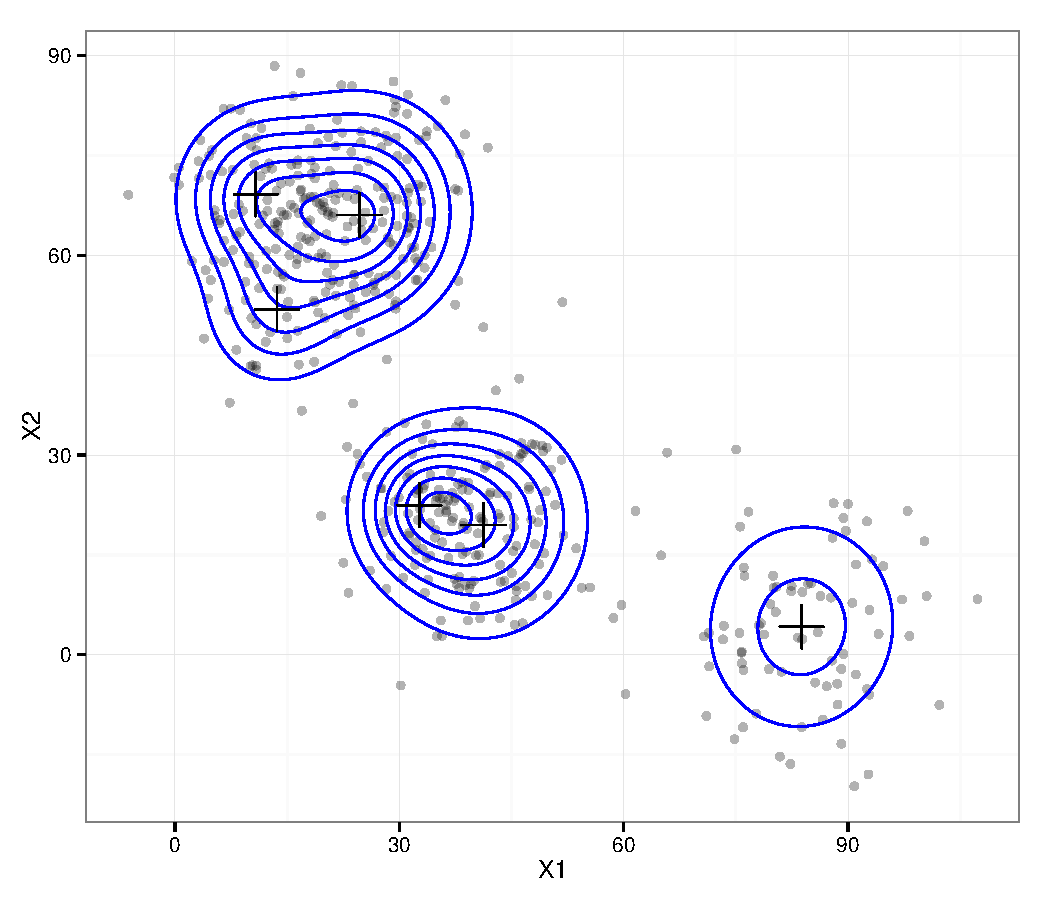
\includegraphics[trim=0cm 0cm 0cm 0cm,width=0.6\textwidth]{figures/partition-example-mixture.pdf} \\
 \end{tabular}
 \caption{Density of a Gaussian mixture with 6 component adjusted to a data set generated from a 3 component Gaussian mixture using R \textsc{MixSim} package with max overlapping of $\check{\omega} = 0.01$. Sample mean of each component is represented by '+'.}\label{ex_mixture}
\end{center}
\end{figure}

Let $I = \{1,2,3,4,5,6\}$. As commented before, any partition of $I$ yields to a feasible final classification using Eq.\ref{cluster_criteria}. For example, the partition 
\[
\mathcal{I}_6 = \{\{1\},\{2\},\{3\},\{4\},\{5\},\{6\}\}
\]
of $I$ yields to a classification where each observation $\m x_i \in \mathbb{R}^2$ is  assigned to the part $\{j\}$ with maximum $\hat{\tau}_{i\{j\}}$. In Figure~\ref{ex_part6} each observation $\m x_i$ is separated according to the assigned part. The isodensity curves for each of the pdf $\hat{f}_{\{j\}} = \phi(\;\cdot\; ; \hat{\m\mu}_j, \hat{\m\Sigma}_j)$, $1\leq j \leq 6$, is included in the graphic. 

%In other words, $\m x_i \in \mathbb{R}^2$ is assigned to cluster labeled
%\[
%\argmax_{j=1}^6 \frac{ \hat{\pi}_{\{j\}} \hat{f}_{\{j\}}(\m x) }{\sum_{\ell=1}^6 \hat{\pi}_{I_\ell} \hat{f}_{I_\ell}(\m x ) }
%\]


%$\hat{f}_{\{j\}}(\;\cdot\;) = \frac{\hat{\pi}_j}{\hat{\pi}_j} f(\;\cdot\;; \hat{\m\mu}_j, \hat{\m\Sigma}_j) = f(\;\cdot\;; \hat{\m\mu}_j, \hat{\m\Sigma}_j)$ for $j = 1,...,6$. Partition $\mathcal{I}_6$ yields to the cluster algorithm where an element $x_i$ is assigned to the part $\{j\}$ of $\mathcal{I}_6$ such that $\hat{\tau}_{i\{j\}}$ is maximum.


\begin{figure}[!h]
\begin{center}
\begin{tabular}{cc}
 %   6 toy mixture
  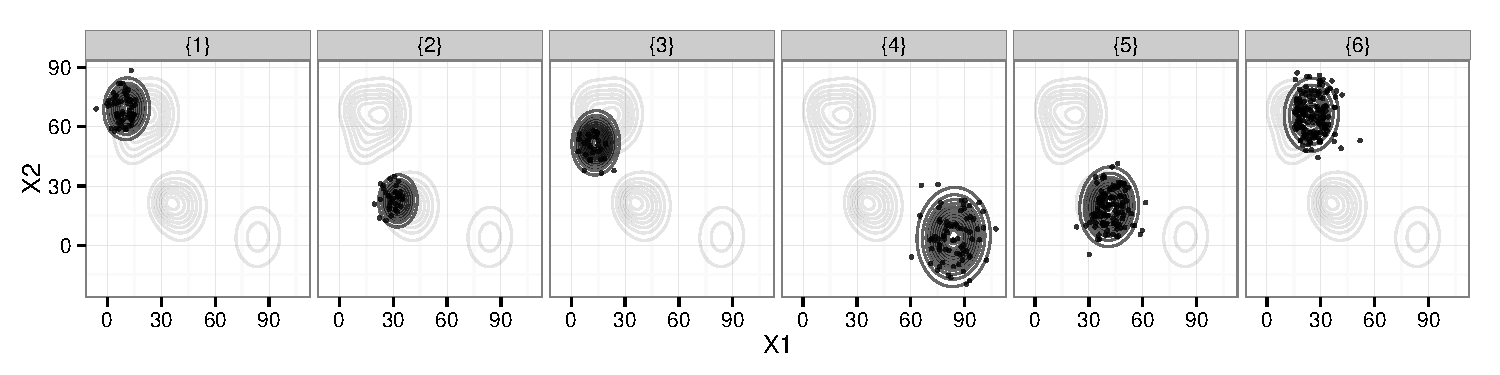
\includegraphics[trim=0cm 0cm 0cm 0cm,width=\textwidth]{figures/partition-example-part6.pdf} \\
 \end{tabular}
 \caption{Classification obtained considering the component partition $\{ \{1\}, \{2\}, \{3\}, \{4\}, \{5\}, \{6\} \}$ with 6 parts in sample $X_{500}$.}\label{ex_part6}
\end{center}
\end{figure}

In contrast, if we consider the partition
\[\mathcal{I}_3 = \{\{1, 3, 6\},\{2, 5\},\{4\}\}\]
which is grouping those components with closest mean, we get the 3 clusters given in Figure~\ref{ex_part3a}. We have included the isodensity curves of pdf $\hat{f}_{\{1,3,6\}}$, $\hat{f}_{\{2, 5\}}$ and $\hat{f}_{\{4\}}$ given by

\[ 
%\left\{ 
\begin{array}{r c l}
\hat{f}_{\{1,3,6\}} & = & \frac{1}{0.52}(0.13 \phi(\;\cdot\; ; \hat{\m\mu}_1, \hat{\m\Sigma}_1) + 0.07 \phi(\;\cdot\; ; \hat{\m\mu}_3, \hat{\m\Sigma}_3) + 0.32 \phi(\;\cdot\; ; \hat{\m\mu}_6, \hat{\m\Sigma}_6)), \\
\hat{f}_{\{2, 5\}} & = &  \frac{1}{0.33}(0.09 \phi(\;\cdot\; ; \hat{\m\mu}_2, \hat{\m\Sigma}_2) + 0.24 \phi(\;\cdot\; ; \hat{\m\mu}_5, \hat{\m\Sigma}_5)), \\
\hat{f}_{\{4\}} & = &\phi(\;\cdot\; ; \hat{\m\mu}_4, \hat{\m\Sigma}_4).
\end{array} 
%\right. 
\]
  


\begin{figure}[!h]
\begin{center}
\begin{tabular}{cc}
  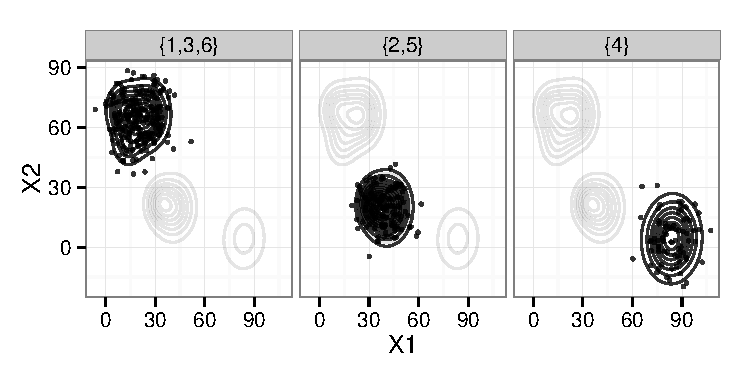
\includegraphics[trim=0cm 0cm 0cm 0cm,width=0.6\textwidth]{figures/partition-example-part3a.pdf} \\
 \end{tabular}
 \caption{Classification obtained considering the component partition $\{\{1, 3, 6 \}, \{2, 5\}, \{5\}\}$ with 3 parts in sample $X_{500}$.}\label{ex_part3a}
\end{center}
\end{figure}

%Finally, suppose that instead of grouping by similar mean, we decide to group by similar covariance matrix. By choosing partition
%\[\mathcal{I}'_3 = \{\{1, 2, 3\},\{4\},\{5, 6\}\},\]
%we end up with the clustering given in Figure~\ref{ex_part3b}.
%
%\begin{figure}[!h]
%\begin{center}
%\begin{tabular}{cc}
%  \includegraphics[trim=0cm 0cm 0cm 0cm,width=0.6\textwidth]{figures/partition-example-part3b.pdf} \\
% \end{tabular}
% \caption{Classifying assigning each observation to a single component}\label{ex_part3b}
%\end{center}
%\end{figure}

Consider the following hierarchical combination of components given by the following sequence of partitions
\begin{equation}
\begin{array}{r c c}
\mathcal{H}(\mathcal{I}) &=& \{ \{\{1\},\{2\},\{3\},\{4\},\{5\},\{6\}\}, \\
   & & \{\{1, 6\},\{2\},\{3\},\{4\},\{5\} \}, \\
   & &    \{\{1, 6, 3\},\{2\},\{4\},\{5\} \}, \\
   & &    \{\{1, 6, 3\},\{2, 5\},\{4 \} \}, \\
    & &   \{\{1, 6, 3\},\{2, 4, 5\} \}, \\
   & &    \{\{1, 2, 3, 4, 5, 6\}\} \}.
\end{array}
\label{hier_ex}
\end{equation}
Each partition from the hierarchical combination of components given by \ref{hier_ex} defines a clustering where each element is classified to one of the parts of each partition. Therefore, a hierarchical combination of components defines a hierarchical clustering structure. Figure~\ref{hierarchical} shows the hierarchical clustering obtained in sample $X_{500}$ using the hierarchical combination of components given in Eq~\ref{hier_ex}. The first partition $\{\{1\},\{2\},\{3\},\{4\},\{5\},\{6\}\}$ defines a clustering with 6 clusters, the partition $\{\{1, 6\}, \{3\},\{2\},\{4\},\{5\} \}$ defines a clustering with 5 clusters, and so on.

\begin{figure}[thbp]
\begin{center}
\begin{tabular}{cc}
  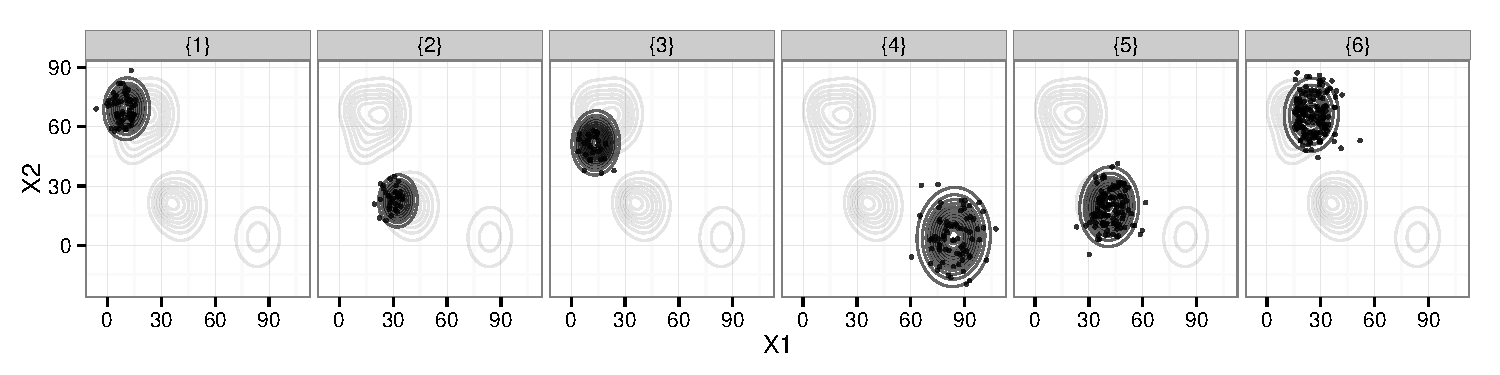
\includegraphics[trim=0cm 0cm 0cm 0cm,width=\textwidth]{figures/partition-example-part6.pdf} \\
    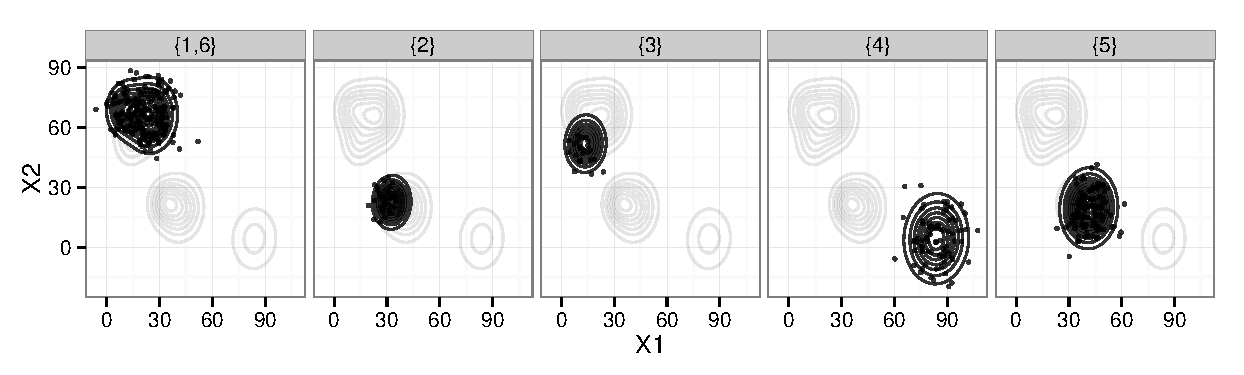
\includegraphics[trim=0cm 0cm 0cm 0cm,width=0.83\textwidth]{figures/partition-example-part5.pdf} \\
      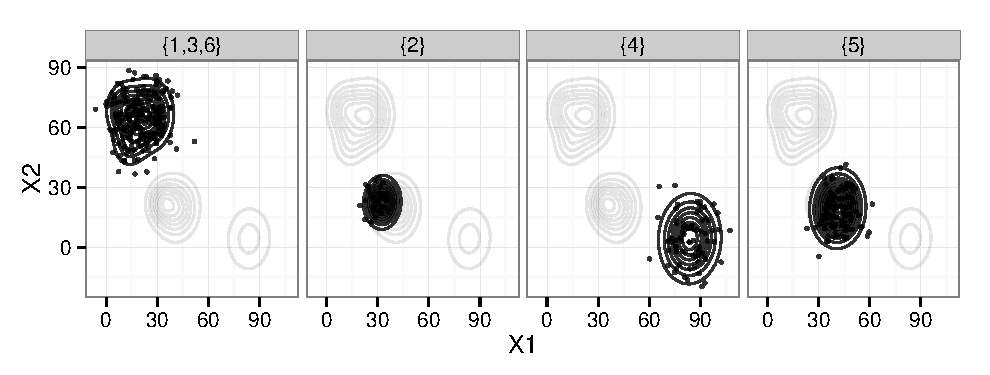
\includegraphics[trim=0cm 0cm 0cm 0cm,width=0.67\textwidth]{figures/partition-example-part4.pdf} \\
        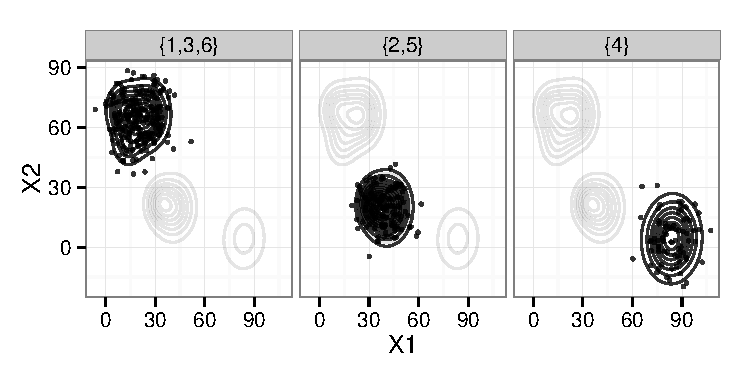
\includegraphics[trim=0cm 0cm 0cm 0cm,width=0.5\textwidth]{figures/partition-example-part3a.pdf} \\
          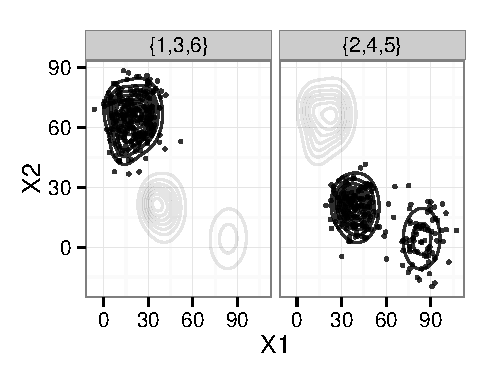
\includegraphics[trim=0cm 0cm 0cm 0cm,width=0.33\textwidth]{figures/partition-example-part2.pdf} \\
            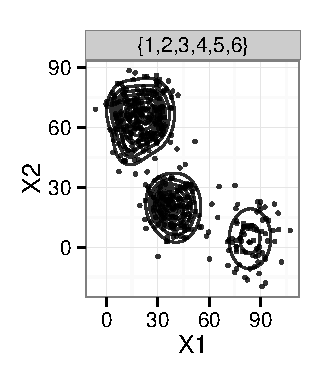
\includegraphics[trim=0cm 0cm 0cm 0cm,width=0.2\textwidth]{figures/partition-example-part1.pdf}
 \end{tabular}
 \caption{Hierarchical cluster obtained by the hierarchical combination of components.}\label{hierarchical}
\end{center}
\end{figure}

In next section we review and propose different methods to decide how to merge the components. More concretely, given a finite mixture we analyse methods to decide how to merge components only using information given by the posterior probabilities $\hat{\tau}_{i \mathcal{I}}$, $1\leq i \leq n$.


%we are not interested in how to decide which of the different partitions in a hierarchical combination of components defines a ``better'' clustering. 

\section{Hierarchical approaches based on posterior probabilities}
\label{old_methods}

%In this section we review different approaches to build a hierarchical combination of components using the information contained in the posterior probabilities $\hat{\tau}_{iI}$. The motivation of this section are: to reformulate the different approaches with the same notation, and to indicate the idea behind this approaches. Moreover, in this section we present a new method to generate a hierarchical combination of components. The new approach is based the log-ratios.

Once a finite mixture distribution is adjusted to a sample $X=\{x_1, \dots, x_n\}$, given a partition $\mathcal{I}_s = \{ I_1, \dots, I_s\}$ we can calculate the posterior probability vector   $\hat{\m\tau}_{i \mathcal{I}_s} = \left( \hat{\tau}_{i I_1} , \dots, \hat{\tau}_{i I_s}  \right)$ for $i$, $1 \leq i \leq n$. 

In this section we show different approaches to combine two parts $I_a$ and $I_b$ from partition $\mathcal{I}_s$ into one part $I_a \cup I_b$. The shown methods only use the information contained in the posterior probability vectors $\{ \hat{\m\tau}_{1 \mathcal{I}_s},\dots, \hat{\m\tau}_{n \mathcal{I}_s} \}$.


\subsection*{Approach based on the total Entropy}

%Let ${\boldsymbol\tau}_1, \dots, {\boldsymbol\tau}_n$ be the probability vectors giving the probability that elements $\textbf{x}_1, \dots, \textbf{x}_n$ belongs to classes $C_1, \dots, C_k$.  

%Once a finite mixture distribution is adjusted to a sample $X=\{x_1, \dots, x_n\}$. Given a partition $\mathcal{I}_s = \{ I_1, \dots, I_s\}$, for each element $\m x_i$ we can calculate the posterior probabilities of $\m x_i$ being classified to each part, obtaining \emph{the posterior probability composition} $\hat{\tau}_{i \mathcal{I}_s} = \left( \hat{\tau}_{i I_1} , \dots, \hat{\tau}_{i I_s}  \right)$ summing up to one. \marginpar{Potser això estaria millor a definicions}

Let $\hat{\m \tau}_{i \mathcal{I}_{s, a \cup b}}$ be the posterior probability vector obtained  after joining the part $I_a$ and $I_b$ from $ \mathcal{I}_s$ into one part $I_{a \cup b}$. Put in other words, $\hat{\m \tau}_{i \mathcal{I}_{s, a \cup b}}$ is the posterior probability vector for the partition
\[
\mathcal{I}_{s, a \cup b} = \left( \mathcal{I}_s \setminus \{ I_a, I_b \} \right) \cup \left\{ \{ i | i \in I_a\cup I_b \} \right\}.
\]

The Entropy of a posterior probability vector $\hat{\m \tau}_{i \mathcal{I}_s}$ is
\[
Ent( \hat{\m \tau}_{i \mathcal{I}_s} ) = \sum_{j=1}^s \hat{\tau}_{i I_j}  log(\hat{\tau}_{i I_j} ).
\]
$Ent( \hat{\m \tau}_{i \mathcal{I}_s} )$ is a convex function with its minimum at $(\frac{1}{s},\dots,\frac{1}{s})$. In terms of posterior probabilities, the minimum is the point where the posterior probability of an observation $x_i$ to be generated from distributions $\hat{f}_{I_1}, \dots, \hat{f}_{I_s}$ is the same when $x_i$ is generated from a finite mixture distribution with pdf given by Eq.~\ref{mixt_part}.

 \cite{baudry2010combining} proposes to merge the components, $I_a$ and $I_b$, such that $\sum_{i=1}^n Ent( \hat{\m \tau}_{i \mathcal{I}_{s, a \cup b}} )$ is minimum. The criteria is equivalent to combine those parts, $I_a$ and $I_b$, such that the difference 
\begin{multline*}
\Delta Ent(\hat{\m \tau}_{i \mathcal{I}_s}, a, b) = \sum_{i=1}^n Ent( \hat{\m \tau}_{i \mathcal{I}_{s, a \cup b}}) - \sum_{i=1}^n Ent( \hat{\m \tau}_{i \mathcal{I}_s}) =  \\ = \sum_{i=1}^n  \left( \hat{\tau}_{i I_{a\cup b}}  log(\hat{\tau}_{i I_{a\cup b}} ) +  \sum_{\substack{j=1 \\
                                                            j \neq a, b}}^s \hat{\tau}_{i I_j}  log(\hat{\tau}_{i I_j} ) \right)  - \sum_{i=1}^n \sum_{j=1}^s \hat{\tau}_{i I_j}  log(\hat{\tau}_{i I_j} ) = \\  =   \sum_{i=1}^n  (\hat{\tau}_{iI_a}+\hat{\tau}_{iI_b}) \log(\hat{\tau}_{iI_a} + \hat{\tau}_{iI_b}) - \sum_{i=1}^n \left\{ \hat{\tau}_{iI_a} \log(\hat{\tau}_{iI_a}) + \hat{\tau}_{iI_b} \log(\hat{\tau}_{iI_b})\right\}
\end{multline*}
is maximum.

It is noteworthy to remark that function $\Delta Ent(\hat{\m \tau}_{i \mathcal{I}_s}, a, b)$ is symmetric, i.e. $\Delta Ent(\hat{\m \tau}_{i \mathcal{I}_s}, a, b) = \Delta Ent(\hat{\m \tau}_{i \mathcal{I}_s}, b, a)$.

To see the effect of the entropy criteria in a simple case , consider the finite mixture
\begin{equation}\label{two_mixture}
f = \pi_a \hat{f}_{I_a} + (1 - \pi_a) \hat{f}_{I_b, \lambda}
\end{equation}
where $\hat{f}_{I_a} = N(0, 1)$ is the normal with mean equal to $0$ and variance $1$, $\hat{f}_{I_b, \lambda} = N(\lambda, 1)$ to be the normal with mean equal to $\lambda$ and variance $1$ and $\pi_a = 0.1, 0.2, 0.3, 0.4, \dots, 0.9$. 

We have approximated the expected value of the total entropy
\[
\mathbb{E}\left[ \Delta Ent\left(
 \left( 
 \frac{\pi_a \hat{f}_{I_a}(\m x)}{\pi_a \hat{f}_{I_a}(\m x) + (1-\pi_a) \hat{f}_{I_b, \lambda}(\m x)}, 
 \frac{(1-\pi_a) \hat{f}_{I_b, \lambda}(\m x)}{\pi_a \hat{f}_{I_a}(\m x) + (1-\pi_a) \hat{f}_{I_b, \lambda}(\m x)} \right), a, b\right) | \m x \sim f \right]
\]
for different values of $\lambda$ and $\pi_a$ by simulating a large sample of observations ($100000$ observations)  following the mixture given by Equation~\ref{two_mixture}.

%We have generated $100000$ observations following mixture given by Equation~\ref{two_mixture} 
%%(we have generated $\pi_a * n$ values from $hat{f}_{I_a}$ and $(1-\pi_a) * n$ values from $hat{f}_{I_b}$), 
%and we have calculate the total Entropy (the mean) for this sample.
In Figure~\ref{fig:mu_varying} (top-left) the total Entropy is represented for $\lambda$, $0 \leq \lambda \leq 3$ and for $\pi_a \in \{ 0.1, 0.2, 0.3, 0.4, 0.5, 0.6, 0.7, 0.8, 0.9\}$. In the plot, because the total entropy is symmetric respect $a$ and $b$, the curves for $\pi_a = 1-\pi_a$ overlap. We can see that for a fixed $\lambda$, the higher confusion appears when $\pi_a = 0.5$.

\begin{figure}[!t]
\centering
\includegraphics[scale=.7]{figure01/fig01.eps}
\caption{$\lambda$ varying}
\label{fig:mu_varying}
\end{figure}

%To ilustrate the total Entropy method consider the following scenario: suppose $\hat{f}_{I_a} = N(0, 1)$ is the standardized normal distribution and let $\hat{f_\lambda}_{I_b} = N(\lambda, 1)$. In Figure~\ref{entropy_plot} the value

%\lambda_{\text{Ent}}(\hat{\tau}_{i \mathcal{I}_s}, I_a, I_b) := 

\subsection*{Directed Estimated misclassification Probabilities (DEMP) approach}

DEMP method was introduced in \cite{hennig2010methods}. The approach proposes to combine the two parts $I_a$ and $I_b$ from $ \mathcal{I}_s$ such that \emph{the probability of classifying an observation generated from component $\hat{f}_{I_a}$ to component $\hat{f}_{I_b}$} is maximum.

To estimate the previous probability,  \cite{hennig2010methods} suggests to use a consistent estimator (DEMP). Using the notation previously introduced, the estimator takes the form
\[
\frac{ \frac{1}{n} \sum_{i=1}^n {\hat{\tau}_{iI_a} \mathbbm{1}\left( \forall j\; \hat{\tau}_{i I_{b}} \geq \hat{\tau}_{iI_j} \right)}}{ \hat{\pi}_{I_a}},
\]
where $\mathbbm{1}\left( \cdot \right)$ is the indicator function. Because $ \hat{\pi}_{I_a} = \frac{1}{n} \sum_{i=1}^n \hat{\tau}_{iI_a}$, the estimator can be rewritten in terms of the posterior probability vector as
\begin{equation}\label{demp_criteria}
DEMP(\hat{\m \tau}_{i \mathcal{I}_s}, a, b) =\frac{ \sum_{i=1}^n {\hat{\tau}_{iI_a} \mathbbm{1}\left( \forall j\; \hat{\tau}_{i I_{b}} \geq \hat{\tau}_{iI_j} \right)}}{\sum_{i=1}^n \hat{\tau}_{iI_a} }.
\end{equation}

In contrast to $\Delta Ent(\hat{\m \tau}_{i \mathcal{I}_s}, a, b)$, $DEMP(\hat{\m \tau}_{i \mathcal{I}_s}, a, b)$ function is not symmetric, and therefore, in general it is different to merge part $I_a$ to part $I_b$ than to merge part $I_b$ to part $I_a$. 

Similarly to the total Entropy, we have approximated the expected value of DEMP function
\[
\mathbb{E}\left[DEMP \left(
 \left( 
 \frac{\pi_a \hat{f}_{I_a}(\m x)}{\pi_a \hat{f}_{I_a}(\m x) + (1-\pi_a) \hat{f}_{I_b, \lambda}(\m x)}, 
 \frac{(1-\pi_a) \hat{f}_{I_b, \lambda}(\m x)}{\pi_a \hat{f}_{I_a}(\m x) + (1-\pi_a) \hat{f}_{I_b, \lambda}(\m x)} \right), a, b\right) | \m x \sim f \right]
\]
for the finite mixture distribution with pdf given by Eq.~\ref{two_mixture}.
In Figure~\ref{fig:mu_varying} (top-right) DEMP is represented for $\lambda$, $0 \leq \lambda \leq 3$ and for $\pi_a \in \{ 0.1, 0.2, 0.3, 0.4, 0.5, 0.6, 0.7, 0.8, 0.9\}$. As commented, in this approach there is no symmetry between $a$ and $b$, we obtain different curves for different values of $\pi_a$. In this case, for $\lambda$ fixed, the higher measure of confusion is obtained when $\pi_a$ is lower. Another feature is that when $\lambda$ tends to zero the curves tends to $0$ if $\pi_a > 0.5$, to $1$ if $\pi_a < 0.5$ and to $0.5$ if $\pi_a = 0.5$. This is due to the fact that when $\hat{f}_{I_a}$ and $\hat{f}_{I_b, \lambda}$ are close enough, deciding if $\hat{\tau}_{i I_{b}}$ is higher to $\hat{\tau}_{i I_{a}}$ depends only on the value of the fixed $\pi_a$.

\subsection*{DEMP modified approach}

In DEMP approach, for an observation generated from a pdf $\hat{f}_{I_a}$, the role played by the indicator function in Equation~\ref{demp_criteria} is to count the number of times the observation is classified to part $I_b$, and therefore, to estimate the probability of classifying an observation to part $I_b$.

\cite{longford2014} proposes a similar approach. Instead of estimating the probability of classifying an observation to part $I_b$, they propose to estimate the probability that the osevation is generated by component $\hat{f}_{I_b}$ taken into an account that the observation has been generated by either $\hat{f}_{I_a}$ or $\hat{f}_{I_b}$. 

In \cite{longford2014} approach, the indicator function in Equation~\ref{demp_criteria} takes the form $\frac{\hat{\tau}_{iI_b}}{\hat{\tau}_{iI_a} + \hat{\tau}_{iI_b}}$. Although in  \cite{longford2014} the estimation $\frac{\hat{\tau}_{iI_b}}{\hat{\tau}_{iI_a} + \hat{\tau}_{iI_b}}$ is obtained by simulating a large amount of observation from component $\hat{f}_{I_a}$, similarly to the DEMP estimator, we can build a direct estimator

\begin{equation}\label{demp_criteria}
DEMP_2(\hat{\m \tau}_{i \mathcal{I}_s}, a, b) =\frac{ \sum_{i=1}^n \hat{\tau}_{iI_a} \hat{\tau}_{iI_b}(\hat{\tau}_{iI_a} + \hat{\tau}_{iI_b})^{-1}  }{\sum_{i=1}^n \hat{\tau}_{iI_a} }.
\end{equation}

Similar to DEMP approach, the modified version of DEMP approach is also not symmetric. An important difference between $DEMP$ and $DEMP_2$ is that $DEMP_2$ only depends on parts  $iI_a$ and $iI_b$ whilst $DEMP$ method is implicitly affected by the other parts.

In Figure~\ref{fig:mu_varying} (bottom-left)  we have approximated the expected value of $DEMP_2$ function
\[
\mathbb{E}\left[DEMP_2 \left(
 \left( 
 \frac{\pi_a \hat{f}_{I_a}(\m x)}{\pi_a \hat{f}_{I_a}(\m x) + (1-\pi_a) \hat{f}_{I_b, \lambda}(\m x)}, 
 \frac{(1-\pi_a) \hat{f}_{I_b, \lambda}(\m x)}{\pi_a \hat{f}_{I_a}(\m x) + (1-\pi_a) \hat{f}_{I_b, \lambda}(\m x)} \right), a, b\right) | \m x \sim f \right].
\]
Observe that the behaviour is similar tending to 0 when function $\hat{f}_{I_a}$ and $\hat{f}_{I_b, \lambda}$ are distant (when $\lambda$ grows). But when they are close (when $\lambda$ tends to 0), each curve tends to the value of $\pi_a$.


%
%The assimetry results in situation where merging $I_a$ to $I_b$ is suitable, but not the other way around. This concept
%
%
%
%The DEMP methods is similar to the method presented in \cite{longford2014}
%
%The function indicator $\mathbbm{1}_{\left[ \forall j\; \hat{\tau}_{i I_{b}} \geq \hat{\tau}_{iI_j} \right]}$ is defined by
%\[
%\mathbbm{1}_{\left[ \forall j\; \hat{\tau}_{i I_{b}} \geq \hat{\tau}_{iI_j} \right]} =
%\left\{\begin{array}{ll}	
%1 & \text{if $\forall j\; \hat{\tau}_{i I_{b}} \geq \hat{\tau}_{iI_j}$}\\
%0 & \text{if $\exists j\; \hat{\tau}_{i I_{b}} < \hat{\tau}_{iI_j}$}
%\end{array}\right.
%\]


%{\color{red} Martin diu que potser hauria de ser $a$ a sota.  Diria que no.}
%{\color{red} Dir què és el DEMP i com mesura la confusió entre b i a. En Hennig parla de misclassification}

\subsection*{The log-ratio approaches}

In the total Entropy approach, the idea of confusion between components is build over the idea that closest the posterior probability vector are from $(\frac{1}{s}, \dots, \frac{1}{s})$ more confused are the components. In contrast, in DEMP and its modified version approaches the idea of confusion is build over the probability of classifying an observation to one component when the observation was generated from another component.
%, and therefore, the approach measures how large is $\hat{\tau}_{iI_b}$. In the modified version of DEMP the measure of how large is $\hat{\tau}_{iI_b}$ is done with respect $\hat{\tau}_{iI_a}$.

Using this two ideas, two new different approaches can be introduced if the idea of confusion between part $I_a$ and $I_b$ is build by comparing the components $\hat{\tau}_{iI_a}$ and $\hat{\tau}_{iI_b}$ relatively inside the posterior probability vector $\hat{\m \tau}_{i \mathcal{I}_s}$. 

The first approach we propose measures the chances of confusing $I_b$ with $I_a$ by considering that if an observation was generated from the probability density function $\hat{f}_{I_a}$, the higher is $\hat{\tau}_{iI_b}$ respect to $\hat{\tau}_{iI_a}$ the higher is the confusion between them. 

%For a partition $\mathcal{I}_s$, the dissimilarity measure $Ent( \hat{\m \tau}_{i \mathcal{I}_s} )$ is minimum when components of the posterior probabilities vector, $\hat{\m \tau}_{i \mathcal{I}}$, is the same, $\m \tau_0 = (\frac{1}{s}, ...,\frac{1}{s})$. The function $Ent( \hat{\m \tau}_{i \mathcal{I}_s} )$ grows as the probability vectors separates from the $\m \tau_0$.
%
%
%The total Entropy approach is an approach which takes into an account 

%The log-ratio approach, proposes the hierarchical combination of components $\mathcal{I}_1, \dots, \mathcal{I}_k$ defined as follows: starting from partition $\mathcal{I}_k = \{\{1\},\dots, \{k\}\}$ at each step the method combines two parts. If at current step we have the partition  $I_1, \dots, I_s$ the two parts, $I_a, I_b$, $1 \leq a,b \leq s$,  to be combined are those that \emph{minimise} log-ratio criterion by

To measure the relative differences between  $\hat{\tau}_{iI_b}$ and $\hat{\tau}_{iI_a}$, we propose to use the log ratio between them, i.e $log( \hat{\tau}_{iI_b}/\hat{\tau}_{iI_a})$. The approach proposes to combine those parts $I_a$ and $I_b$ maximising the following criteria, 

\[
LOG(\hat{\m \tau}_{i \mathcal{I}_s}, a, b) = \frac{\sum_{i=1}^n  \hat{\tau}_{iI_a}  \log( \frac{ \hat{\tau}_{iI_b} }{ \hat{\tau}_{iI_a} })}{\sum_{i=1}^n  \hat{\tau}_{iI_a} }.
\]


The norm of a posterior probability vector, $\| (\hat{\tau}_{iI_a}, \hat{\tau}_{iI_b}) \|$  as defined in ({\color{red} Posar cita correcte, no crec que sigui l'Aitchison qui defineixe la norma}) \citep{aitchison1986statistical} is
\[
\left\| (\hat{\tau}_{iI_a}, \hat{\tau}_{iI_b}) \right\| = \log (\frac{ \hat{\tau}_{iI_b} }{ \hat{\tau}_{iI_a} })^2.
\]
The norm $\| (\hat{\tau}_{iI_a}, \hat{\tau}_{iI_b}) \|$ measures how far is the posterior probability vector $(\hat{\tau}_{iI_a}, \hat{\tau}_{iI_b})$ of the posterior probability vector $(\frac{1}{2}, \frac{1}{2})$.


With the new geometric notion, the second approach follows from the idea that if $I_a$ and $I_b$ are easy to confuse, we expect $\| \left( \hat{\tau}_{iI_a}, \hat{\tau}_{iI_b} \right) \|$ to be low. So, we propose to combine those parts $I_a$ and $I_b$ maximising the following criteria, 
\[
%LOG_2(\hat{\m \tau}_{i \mathcal{I}_s}, a, b) = \frac{\sum_{i=1}^n  \hat{\tau}_{iI_a}  ( -\log( \frac{ \hat{\tau}_{iI_b} }{ \hat{\tau}_{iI_a} })^2 )}{\sum_{i=1}^n  \hat{\tau}_{iI_a} }.
LOG_2(\hat{\m \tau}_{i \mathcal{I}_s}, a, b) = - \sum_{i=1}^n  \log( \frac{ \hat{\tau}_{iI_b} }{ \hat{\tau}_{iI_a} })^2.
\]

%$\hat{\tau}_{iI_a} > \hat{\tau}_{iI_b}$, and therefore, similarly to the Entropy approach, using the distance $d_{\mathcal{A}}(\m x,\m y)$, the log-ratio approach is measuring how different is the posterior probability vector $(\hat{\tau}_{iI_a}, \hat{\tau}_{iI_b})$ of $(\frac{1}{2}, \frac{1}{2})$.
%
%The norm of the subcomposition  $(\hat{\tau}_{iI_a} ,\hat{\tau}_{iI_b})$ measures how far is the sub composition of sub composition $(\frac{1}{2}, \frac{1}{2})$, and it can be used to measure the confusion between parts $I_a$ and $I_b$. 




\begin{figure}[!h]
\centering
\includegraphics[scale=.6]{figure01/fig02.eps}
\caption{$\lambda$ varying {\color{red} Aquesta figura la treuria, no dona la noció de distancia que volem donar.}}
\label{fig:mu_varying_logit}
\end{figure}

The approximation of the expected value of $LOG$ function
\[
\mathbb{E}\left[LOG \left(
 \left( 
 \frac{\pi_a \hat{f}_{I_a}(\m x)}{\pi_a \hat{f}_{I_a}(\m x) + (1-\pi_a) \hat{f}_{I_b, \lambda}(\m x)}, 
 \frac{(1-\pi_a) \hat{f}_{I_b, \lambda}(\m x)}{\pi_a \hat{f}_{I_a}(\m x) + (1-\pi_a) \hat{f}_{I_b, \lambda}(\m x)} \right), a, b\right) | \m x \sim f \right],
\]
is shown in Figure~\ref{fig:mu_varying} (top-right). For $\lambda$ fixed, it shows a similar behaviour as $DEMP$ and $DEMP_2$, that is, lower the $\pi_a$ values, the higher the confusion is. In Figure~\ref{fig:mu_varying_logit} we have represented the inverse of the logit of the expected value.



%%\[
%%\frac{\sum_{i=1}^n \mathbbm{1}_{\left[ \forall j\; \hat{\tau}_{i I_{a}} \geq \hat{\tau}_{iI_j} \right]} \log( \frac{ \hat{\tau}_{iI_a} }{ \hat{\tau}_{iI_b} })}{\sum_{i=1}^n \mathbbm{1}_{\left[ \forall j\; \hat{\tau}_{i I_{a}} \geq \hat{\tau}_{iI_j} \right]}}.
%%\]
%
%
%
%{\color{red} Dir que la mesura és igual a la mitjana de les distàncies entre la subcomposició $(\tau_a, \tau_b)$ i $(0.5,0.5)$ per les observacions classificades a $a$.}
%
%\begin{itemize}
%\item a local measure of how possible is to confuse $I_b$ with $I_a$ depending on each observation $\m x_i$, $\log( \frac{ \hat{\tau}_{iI_a} }{ \hat{\tau}_{iI_b} })$, and
%\item a measure of how associated is an observation $\m x_i$ to cluster $I_a$, $\mathbbm{1}_{\left[ \forall j\; \hat{\tau}_{i I_{a}} \geq \hat{\tau}_{iI_j} \right]}$.
%\end{itemize}

\section{Unifying the approaches}
\label{confusion}

In previous section, we have presented different approaches to merge the components of a finite mixture. Some of them were approaches presented by other authors, and the others, up to our knowledge were presented for the first time. In this section, we consider the previous methods into a more general setting.

Consider a posterior probability vector $\hat{\m \tau}_{i \mathcal{I}_s}$. Let $\lambda(\hat{\m \tau}_{i \mathcal{I}_s}, a, b)$  be a function measuring the chances that an observation $\m x_i$ coming from $\hat{f}_{I_a}$ is classified to part $I_a$. In previous section we have seen different possibilities for this function:
\begin{itemize}
\item $\lambda(\hat{\m \tau}_{i \mathcal{I}_s}, a, b) = (\hat{\tau}_{iI_a}+\hat{\tau}_{iI_b}) \log(\hat{\tau}_{iI_a} + \hat{\tau}_{iI_b}) - \hat{\tau}_{iI_a} \log(\hat{\tau}_{iI_a}) + \hat{\tau}_{iI_b} \log(\hat{\tau}_{iI_b})$,
\item $\lambda(\hat{\m \tau}_{i \mathcal{I}_s}, a, b) =\mathbbm{1}\left( \forall j\; \hat{\tau}_{i I_{b}} \geq \hat{\tau}_{iI_j} \right)$, 
\item $\lambda(\hat{\m \tau}_{i \mathcal{I}_s}, a, b) =\hat{\tau}_{iI_b}(\hat{\tau}_{iI_a} + \hat{\tau}_{iI_b})^{-1}$, 
\item $\lambda(\hat{\m \tau}_{i \mathcal{I}_s}, a, b) =\log( \frac{ \hat{\tau}_{iI_b} }{ \hat{\tau}_{iI_a} })$.
\end{itemize}
Moreover, let $\omega(\hat{\m \tau}_{i \mathcal{I}_s}, a)$ be a function measuring the representativeness of observation $x_i$ of part $I_a$. For example:
\begin{itemize}
\item $\omega(\hat{\m \tau}_{i \mathcal{I}_s}, a) = const$,
\item $\omega(\hat{\m \tau}_{i \mathcal{I}_s}, a) =  \hat{\tau}_{iI_a}$ or
\item $\omega(\hat{\m \tau}_{i \mathcal{I}_s}, a) = \mathbbm{1}\left( \forall j\; \hat{\tau}_{i I_{a}} \geq \hat{\tau}_{iI_j} \right)$.
\end{itemize}
In the first example, each observation represents part $I_a$ equally. In the last example, only observations classified to part $I_a$ represent the element of part $I_a$.

With functions $\lambda(\hat{\m \tau}_{i \mathcal{I}_s}, a, b)$ and $\omega(\hat{\m \tau}_{i \mathcal{I}_s}, a)$ we can consider the following approach. For a partition $\mathcal{I}_s = \{ I_1, \dots, I_s\}$ let $\hat{\m\tau}_{i \mathcal{I}_s} = \left( \hat{\tau}_{i I_1} , \dots, \hat{\tau}_{i I_s}  \right)$ for $i$, $1 \leq i \leq n$, be the posterior probability vectors calculated from sample $X$. With the set $\hat{\m\tau}_{i \mathcal{I}_s}$ consider the following approach. Given partition $\mathcal{I}_s$ merge the two parts $I_a$ and $I_b$, into one part $I_a \cup I_b$ which maximise
\begin{equation}\label{unifying_equation}
\frac{\sum_{i=1}^n \omega(\hat{\tau}_{i \mathcal{I}_s}, I_a) \lambda(\hat{\tau}_{i \mathcal{I}_s}, I_a, I_b)}{\sum_{i=1}^n \omega(\hat{\tau}_{i \mathcal{I}_s}, I_a) }.
\end{equation}

%In this section, we extend the ideas that motivate the log-ratio algorithm to a general framework. We consider a local measure given by function $\lambda(\hat{\m\tau}_{i \mathcal{I}}, I, J)$ of how similar are the clusters given by part $I$ and part $J$ in $\m x_i$, and a measure of how associated is an observation $\m x_i$ to the cluster given by part $I$, $\omega(\m x_i, I)$. This general approach proposes the hierarchical combination of components $\mathcal{I}_1 \dots, \mathcal{I}_k$ defined as follows: starting from partition $\mathcal{I}_k = \{\{1\},\dots, \{k\}\}$ at each step the method combine two parts. If at current step we have the partition  $I_1, \dots, I_s$ the two parts, $I_a, I_b$, $1 \leq a,b \leq s$,  to be combined are those that \emph{minimise} the general criterion given by


The Equation~\ref{unifying_equation} allows to model all the approaches given in previous section,
\begin{itemize}
\item Entropy
\begin{itemize}
\item $\omega(\hat{\m \tau}_{i \mathcal{I}_s}, a) = const$
\item $\lambda(\hat{\m \tau}_{i \mathcal{I}_s}, a, b) = (\hat{\tau}_{iI_a}+\hat{\tau}_{iI_b}) \log(\hat{\tau}_{iI_a} + \hat{\tau}_{iI_b}) - \hat{\tau}_{iI_a} \log(\hat{\tau}_{iI_a}) + \hat{\tau}_{iI_b} \log(\hat{\tau}_{iI_b})$
\end{itemize}

\item $DEMP$
\begin{itemize}
\item $\omega(\hat{\m \tau}_{i \mathcal{I}_s}, a) = \hat{\tau}_{iI_a}$
\item $\lambda(\hat{\m \tau}_{i \mathcal{I}_s}, a, b) = \mathbbm{1}\left( \forall j\; \hat{\tau}_{i I_{b}} \geq \hat{\tau}_{iI_j} \right)$
\end{itemize}

\item $DEMP_2$
\begin{itemize}
\item $\omega(\hat{\m \tau}_{i \mathcal{I}_s}, a) = \hat{\tau}_{iI_a}$
\item $\lambda(\hat{\m \tau}_{i \mathcal{I}_s}, a, b) = \hat{\tau}_{iI_b}(\hat{\tau}_{iI_a} + \hat{\tau}_{iI_b})^{-1}$
\end{itemize}

\item $Log$
\begin{itemize}
\item $\omega(\hat{\m \tau}_{i \mathcal{I}_s}, a) = \hat{\tau}_{iI_a}$
\item $\lambda(\hat{\m \tau}_{i \mathcal{I}_s}, a, b) = \log( \frac{ \hat{\tau}_{iI_b} }{ \hat{\tau}_{iI_a} })$
\end{itemize}
\end{itemize}



{\color{red} Aquest paràgraf està molt "xulo". Però crec que cal haver-ne parlat abans quan s'ha presentat els índexos. 
Vull dir, quan es presetna cada índex aniria bé explicar la idea "geomètrica" que ha pensat l'autor (Henning,  Baudry, Comas). Després aquí, aquest aparta xulo s'entendrà molt més. }


The three approaches(Entropy, DEMP, Log) give us three different possible definition for functions $\lambda(\hat{\tau}_{i \mathcal{I}_s}, I_a, I_b)$ and $\omega(\hat{\tau}_{i \mathcal{I}_s}, I_a)$. For the function $\lambda(\hat{\tau}_{i \mathcal{I}_s}, I_a, I_b)$ the entropy approach considers that the more the confusion is between two parts the higher is the difference between the entropy considering the partition with the two part together and merged. The way the confusion is defined by the DEMP approach is more subtle, it states that the higher the confusion between two parts the higher the number of observations not classified to one part. The log-ratio approach relates the confusion respect to the magnitude of the log-ratio. For the function $\omega(\hat{\tau}_{i \mathcal{I}_s}, I_a)$, the entropy approach weigths equally the local information of each observation to decide if $I_a$ should be merged to $I_b$. By contrast, the DEMP and Log approach weigths the observation according to the probability of pertinence to $I_a$. 
%Finally, the log-ratio algorithm weigths with respect the final pertinence to $I_a$.

\begin{table}[!ht]
\begin{tabular}{c  c | >{\centering}m{0.7in} | >{\centering}m{0.7in} | >{\centering}m{0.7in} | m{0in}}
 & \multicolumn{1}{c}{} & \multicolumn{3}{c}{$\omega(\boldsymbol\tau_i, a)$} &\\

 & \multicolumn{1}{c}{} & \multicolumn{1}{c}{} & \multicolumn{1}{c}{} & \multicolumn{1}{c}{} & \multicolumn{1}{c}{}\\

 & \multicolumn{1}{c}{} & \multicolumn{1}{c}{1} & \multicolumn{1}{c}{$\tau_{ia}$} & \multicolumn{1}{c}{$\mathlarger{\mathbbm{1}}\left\{  \forall \ell\; \; \tau_{ia} \geq \tau_{i\ell}  \right\}$} &\\ \cline{3-5} 

& $\large\substack{(\tau_{i a}+\tau_{i b}) \log(\tau_{i a} + \tau_{i b}) - \\ - \tau_{i a} \log(\tau_{i a}) - \tau_{i b} \log(\tau_{i b}) }$ & $Entropy$ &  &  &\\[5em] \cline{3-5}

\rotatebox[origin=c]{90}{$\lambda(\boldsymbol\tau_i, a, b)$} & $\mathlarger{\mathbbm{1}}\left\{  \forall \ell \; \tau_{hb} \geq \tau_{h\ell}  \right\}$ & & $DEMP$  & -- & \\[5em] \cline{3-5}

& ${\tau_{i b}}({\tau_{i a}+\tau_{i b}})^{-1}$ &  &  $DEMP_2$ &  &\\[5em] \cline{3-5}

& $\log{\tau_{i b} / \tau_{i a}}$ & & $Log$ &   &\\[5em] \cline{3-5}

& $\tau_{i b}$ &  &  &  &\\[5em] \cline{3-5}

\end{tabular}
\caption{Different combinations of score functions}
\end{table}

{\color{red} Seguir l'exemple de les 6 components i estudiar com es calculen els tres indexos en un determinat pas de la jerarquia. Per exemple, quan es decideix fusion el {3} amb el {1,6}. O alguna cosa simila. Preparar-ho pel CoDaWor juntament amb un cas d'estudi final}

{\color{red} Posar lo de Kullback Leibler prenent tau i logratio. Donar la idea que no només és una unificació de tres index si no que una generalització.}

\section{Simulation}

\begin{itemize}
\item For a fixed value of $\omega$, we repeat $1000$ the following process:
\begin{itemize}
\item Generate a sample of size $n=500$ with $D=5$ coordinates coming from the gaussian mixture with $3$ components whose components have maximum overlapping $\omega$.
\item Fit a mixture
\end{itemize}


\end{itemize}
%\section{Fitting a hierarchical model  to a mixture of gaussian distributions}

%Using Equation~\ref{unifying_equation} different methods can be proposed.

\begin{figure}[!h]
\centering
\includegraphics[width=\textwidth]{figure02/linesAR.pdf}
\caption{$\lambda$ Adjusted Rand index results.}
\label{fig:mua}
\end{figure}

\begin{figure}[!h]
\centering
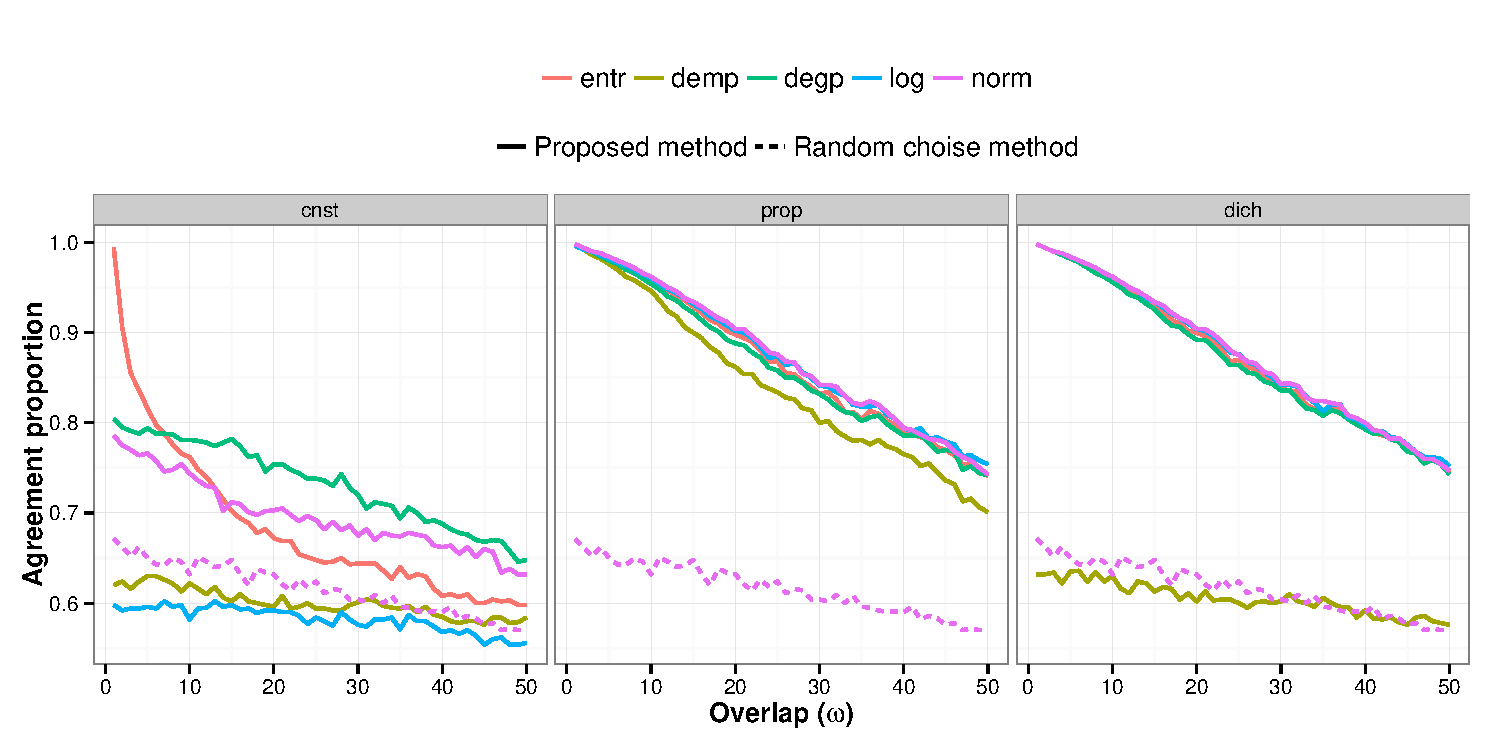
\includegraphics[width=\textwidth]{figure02/linesagreement.pdf}
\caption{$\lambda$ Agreement proportion results.}
\label{fig:mub}
\end{figure}


\bibliographystyle{apalike}
\bibliography{tex/combining_mixtures}{}

\end{document}
